\chapter{Preliminares}

\section{Construcciones básicas}
\subsection{Categorías}
\begin{definition}[Categoría]
 Una categoría $\C$ consta de los siguientes datos: 
    \begin{enumerate}
        \item[$\bullet$]  Una clase (no necesarimente un cojunto) de objetos $\Ob(\C)$, y una clase de morfismos $\Mor(\C)$. 
        \item[$\bullet$]  A cada par de objetos $X,Y\in \Ob(\C)$ le  
        corresponde  una clase de morfismos (flechas) de $X$ en $Y$, que se denotará por $\Mor_\C(X,Y)$.
        \item[$\bullet$]  Para cada terna de objetos $X,Y,Z\in\Ob(\C)$ está definida una función llamada composición 
	\begin{eqnarray*}
	\Mor_\C(X,Y)\times \Mor_\C(Y,Z)&\rightarrow & \Mor_\C(X,Z)\\
 	(f,g)&\mapsto& g\circ f.
	\end{eqnarray*}
    \end{enumerate}
Además, estos datos satisfacen las siguientes propiedades
\begin{enumerate}
    \item[$\bullet$] La composición es asociativa, es decir, $h\circ(f\circ g)=(h\circ f)\circ g$.
    \item[$\bullet$]  Para cada objeto $X\in \Ob(\C)$ existe un morfismo $Id_X\in \Mor_\C(X,X)$ tal que $f\circ Id_X=Id_X\circ f.$
\end{enumerate}
\end{definition}
Para cualesquiera $X,Y\in\Ob(C)$, una manera de denotar los morfismos de $X$ en $Y$ es por $\Mor_\C(X,Y)$ tal como se muestra en la definición anterior. Sin embargo, también es común denotarlo por  $\Hom_\C(X,Y)$ o $\C(X,Y)$.\\ A continuación se presentan algunos de los ejemplos clásicos de categorías.
\begin{ejp}
\text{ }
    \begin{enumerate}
        \item $\Con$ denota la categoría de conjuntos cuyos objetos son conjuntos y, tiene como morfismos las funciones entre conjuntos. La composición entre morfismos está bien definida, y el morfismo identidad es la función identidad. 
        \item $\Vect_k$ es la categoría que tiene por objetos espacios vectoriales sobre un campo $k$ y, como morfismos transformaciones lineales entre espacios vectoriales.
        \item Sean $A$ y $B$ conjuntos parcialmente ordenados. Un morfismo de $A$ a $B$ es una función monótona (creciente). Esto es, para cualesquiera $a,b\in A$, $a\leq b$ implica que $f(a)\leq f(b)$. Así, los conjuntos parcialmente ordenados junto con sus morfismos constituyen la categoría $\Pos$. Un caso ``más general'' es el siguiente: para cualesquiera dos conjuntos parcialmente ordenados $A$ y $B$, estos se pueden ver como categorías, por lo que un morfismo de $A$ a $B$ no es más que un funtor. 
        \item Algunos ejemplos más son los siguientes: $\Top$ es la categoría de espacios topológicos con morfismos las funciones continuas. Por otro lado, tenemos las categorías de grupos y la categoría de anillos con unidad, $\Grp$ y $\Ring$, cuyos morfismos son homomorfismos de grupos y homomorfismos de anillos, respectivamente. 
    \end{enumerate}
\end{ejp}
\begin{definition}[Categoría pequeña]
    Una categoría $\C$ se dice \emph{pequeña} si la clase objetos $\Ob(\C)$ y la clase de morfismos $\Mor(\C)$ es un conjunto.  
\end{definition}
\begin{definition}[Objeto final/inicial] Sea $\C$ una categoría. Un objeto $T\in\Ob(\C)$ es \emph{final} si para cualquier otro objeto $X\in \Ob(\C)$ existe un único morfismo $f:X\to T$. Análogamente, un objeto $I\in\Ob(\C)$ se dice \emph{inicial} si para cualquier $X\in\Ob(\C)$ existe un único morfismo $g:I\to X$. 
\end{definition}
\begin{prop}
Los objetos finales/inicales, si existen, son únicos salvo 
isomorfismo único \cite{mac2013categories}.
\end{prop}
\subsection{Principio de dualidad}
De la definición de objeto inicial y final, es común pensar que uno es la parte ``dual'' del otro. En la práctica, es común encontrarse con ciertas propiedades que satisface una categoría, sin embargo, muchas de estas propiedades tienen una noción ``dual'' en el sentido de que también se siguen cumpliendo aún cuando se cambia la dirección de las flechas entre los objetos. Esto motiva a la siguiente definición.
\begin{definition}[Categoría opuesta] Sea $\C$ una categoría. Se define la \emph{categoría opuesta} de $\C$, denotada por $\C^{\op}$, como la categoría cuyos objetos son los mismos que los de $\C$, i.e., $\Ob(\C^{\op})=\Ob(\C)$, pero sus morfismos van en sentido opuesto, esto es, si $X^{\op}=X,Y=Y^{\op}\in\C^{\op}$, una flecha $f^{\op}:X^{\op}\rightarrow Y^{\op}$ en $\C^{\op}$ es una flecha $f:Y\rightarrow X$  en $\C$. De este modo se tiene que   
    \[\Mor_{\C^{\op}}(X,Y)=\Mor_\C(Y,X).\]
\end{definition}
Además, la ley de composición está dada por $f^*\circ g^*=(g\circ f)^*$. Observemos  que  $(\C^{\op})^{\op}=\C$, es decir,  la categoría opuesta de $\C^{\op}$ es la categor\'ia original.\\
La importancia de trabajar con la categoría dual reside en el siguiente resultado conocido como el principio de dualidad. 
\begin{theo}
    Supongamos la validez, en toda categoría, de un enunciado que expresa la existencia de algún objeto o morfismo o la igualdad de algunas composiciones. Entonces, el \textquotedbl enunciado dual \textquotedbl, que se obtiene al voltear la dirección de las flechas y al sustituir cada composición $f\circ g$ por $g\circ f$ en el enunciado original, es también válido en  toda categoría.
\end{theo}
\subsection{Funtores}
\begin{definition}[Funtor covariante]
Sean $\A$ y $\B$ categorías. Un funtor \emph{covariante} $F:\A\rightarrow\B$ consiste de lo siguiente:
\begin{enumerate}
\item[$\bullet$] Una asignación en objetos: $F:\Ob(\A)\rightarrow \Ob(\B)$.
\item[$\bullet$] Para cada $X,Y\in\Ob(\A)$ se tiene una asignación
\[F: \mathrm{Mor}_\mathcal{A}(X,Y)\rightarrow \mathrm{Mor}_\mathcal{B}(F(X),F(Y)).\]	
\end{enumerate}
Que satisfacen las siguientes propiedades.
\begin{enumerate}
		\item[$\bullet$] $F$ respeta la identidad:	
		\[ F(Id_X)=Id_{F(X)}. \]
		\item[$\bullet$] Respeta la composición:
		\[ F(g\circ f) = F(g)\circ F(f).\]
\end{enumerate}
\end{definition}
\begin{definition}[Funtor contravariante] Diremos que un funtor es \emph{contravaruiante} si corresponde a un funtor covariante de la forma $F:\A^\op\rightarrow\B$.
\end{definition}
De la definición anterior, se tiene que si $F:\A\to\B$ y $G:\B\to\C$ son funtores, entonces su composición $G\circ F:\A\to\C$ está dada por
 \begin{enumerate}
     \item[i)] El compuesto en objetos, 
     \[(G_0\circ F_0):A_0\to C_0,\quad A_0\in\A,\text{ } C_0\in\C.\]
     \item[ii)] Para cada $A,B\in\mathcal{C}$, el compuesto en morfismos
     \[(G_{F(A),F(B)}\circ F_{A,B}):\Mor_\A(A,B)\to\Mor_\C(G(F(A)),G(F(B))).\]
 \end{enumerate}
 Con esto en mente, definimos lo siguiente.
\begin{definition}
Sean $\A$ y $\B$ categorías. Diremos que $\A$ y $\B$ son \emph{isomorfas} si existen funtores $F:\A\rightarrow \B$ y $G:\B\rightarrow \A$ tal que uno es inverso del otro, i.e., $F\circ G= \id_\B$ y $G\circ F=\id_\A$.
\end{definition}
\todo{Añadir ejemplos}
	
\subsection{Transformaciones naturales}
La manera de relacionar objetos de una categoría es mediante sus morfismos. Como vimos anteriormente, dadas dos categorías es posible obtener información de una a partir de la otra mediante un funtor. En esta sección, estamos interesados en estudiar transformaciones naturales, que a grandes rasgos, estas se pueden entender como morfismos entre funtores.
\begin{definition}[Transformación natural] Sean $F,G:\A\to\B$ funtores. Un \emph{transformación natural} es una tupla $(F,\eta, G)$, en donde $\eta:F\to G$ es una colección de morfismos $\eta_A:F(A)\to G(A)$ en $\B$ tal que 
\begin{enumerate}
    \item Para cada $A\in\mathcal{A}$, se tiene que $\eta_\mathcal{A}:F(A)\rightarrow G(A)$.
    \item Para toda $f\in\A(A,B)$, el siguiente diagrama 
    \begin{center}
	\par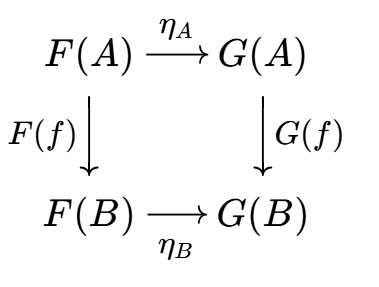
\includegraphics[height=0.22\textwidth]{diagram1.5.1.png}
    \end{center}
    conmuta.
\end{enumerate}
\end{definition}
Si $\eta_A:F(A)\to G(A)$ es un isomorfismo para todo $A\in\Ob(\A)$, diremos que $\eta:F\to G$ es un \emph{isomorfismo natural}, el cual denotamos por $F\cong G$. De esto se sigue que  $\eta^{-1}:F\to G$ dada por $\eta^{-1}_A=(\eta_A)^{-1}$ también es una transformación natural.
\begin{ejp}
Sea $\A$ una categoría pequeña y $\B$ una categoría arbitraria. La categoría de funtores, denotada por $\Fun(\mathcal{A},\mathcal{B})$ (o algunas veces también es denotada por $[\mathcal{A},\mathcal{B}]$), tiene como objetos funtores con dominio $\mathcal{A}$ y codominio $\mathcal{B}$. Para cualesquiera dos funtores en $\Fun(\A,\B)$, un morfismo entre estos es una transformación natural.
 \end{ejp}
 \begin{definition}[Funtor representable] Sea $\C$ una categoría y $F:\C\to\Con$ un funtor. Diremos que $F$ es \emph{representable} si existe un isomorfismo natural entre $F$ y $\Hom(A,-)$, para algún $A\in \Ob(\C)$. En este caso, se dice que $F$ es representado por $A$.
 \end{definition}
Una caracterización de cuando un funtor es representable es la siguiente (veáse \cite{mac2013categories}). Un funtor $F:\C^\op\to\Con$ es representable si, y solo si,  $F\cong h_X$ para algún $X\in\Top$. Esto motiva a enunciar uno  de los resultados de mayor importancia en la teoría de categorías.\todo{Añadir en los ejemplos de funtores el funtor de puntos $h_X$.}
 \begin{lema}[Lema de Yoneda] Sea $F:\C\to\Con$ un funtor. Dado el funtor $\Hom(C,-)$, se tiene que el morfismo
 \begin{eqnarray*}
     \varphi:\Hom(\Hom(A,-))&\to& F(A)\\
     \eta&\mapsto& \eta_A
 \end{eqnarray*}
es un isomorfismo.
 \end{lema}

\section{Límites/colímites}
\subsection{Límites}

\begin{definition}
    Sea $F:\A\to\C$ un funtor. Un \emph{cono} sobre $F$ es una pareja $(C,\langle P_A\rangle_{A\in\A})$ que consiste de lo siguiente:
    \begin{enumerate}
        \item Un objeto $C\in\C$,
        \item Para cada objeto $A\in\A$, se tiene una flecha $(P_A:C\to FA)\in\C$ tal que, para cada flecha $\left(A\xrightarrow{\alpha}A'\right)\in\A$, el siguiente diagrama 
        \begin{figure}[h!]
            \centering
            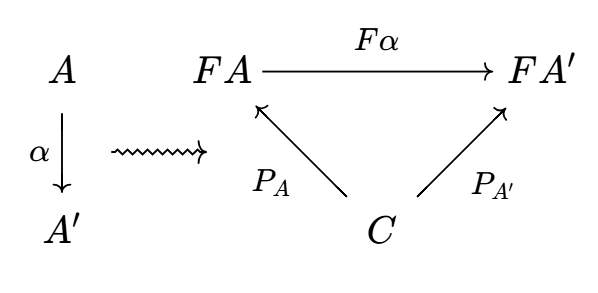
\includegraphics[width=0.35\linewidth]{img/diagrama1.png}
        \end{figure}
        es sólido en $\C$
    \end{enumerate}
\end{definition}
\begin{definition}
    Sea $F:\A\to\C$ un funtor. Un \emph{límite} sobre $F$ es un cono $(L,\langle P_A\rangle_{A\in\A})$ sobre $F$ con la siguiente propiedad: para cualquier otro cono $(M,\langle q_A\rangle_{A\in\A})$ sobre $F$, existe un único morfismo $m:M\to L$ tal que, para todo $A\in \A$, el diagrama
\begin{figure}[H]
    \centering
    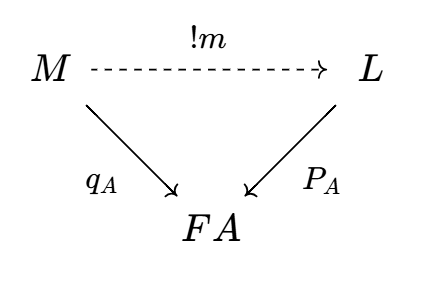
\includegraphics[width=0.3\linewidth]{img/diagrama2.png}
\end{figure}
    conmuta. Esto es, $q_A=P_A\circ m$, para todo $A\in \A$.
\end{definition}
A los morfismos $(P_A:L\to FA,\quad A\in \A)$ se les llama \emph{proyecciones}, y al límite de $F$ se denota como $\varprojlim_{A\in\A} FA$.
\begin{lema}
    El límite de un funtor $F:\A\to\C$, cuando existe, es único salvo isomorfismo natural.
\end{lema}
\begin{proof}
\todo{Pendiente}
\end{proof}
\begin{lema}
    Sea $(L,\langle P_A\rangle_{A\in \A})$ el límite de $F:\A\to\C$. Son morfismos son iguales $\left(
M \overset{f}{\underset{g}{\rightleftarrows}} L \right)\in\C$ si, para todo $A\in \A$, $P_Af=P_Ag$.
\end{lema}
\begin{proof}
    La demostración es inmediata de la propiedad universal del límite. 
\end{proof}

A continuación, se muestran algunos de los ejemplos de límites. 
\begin{ejp}\label{ejp:lim}\text{ }
    \begin{enumerate}
        \item Sea $\A$ una categoría vacía, $\C$ una categoría y $F:\A\to\C$ un funtor. Entonces, el límite de $F$ es un objeto $C\in\Ob(\C)$ tal que, para todo $C'\in\Ob(\C)$, existe un único morfismo $C'\to C$. Es decir, $C$ es el objeto final de $\C$.
        \item Sea $\T$ una categoría con  objetos $\bullet$, $*$, y  $F:\T\to \C$ un funtor. Entonces, un límite para $F$ es 
        \begin{figure}[H]
            \centering
            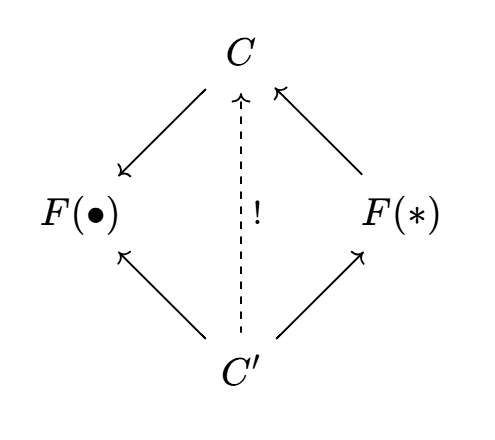
\includegraphics[width=0.3\linewidth]{img/diagrama5.png}
        \end{figure}
        Por lo tanto, $C$ define un producto para $F(\bullet)$ y $F(*)$, el cual denotamos como $C=F(\bullet)\times F(*)$.
        \item Sea $\L$ la categoría que consiste de los objetos $\bullet$ y $*$, dos flechas paralelas de $\bullet$ a $*$, y las respectivas identidades. Sea $F:\L\to\C$ un funtor. De manera diagramática tenemos lo siguiente
        \begin{figure}[H]
            \centering
            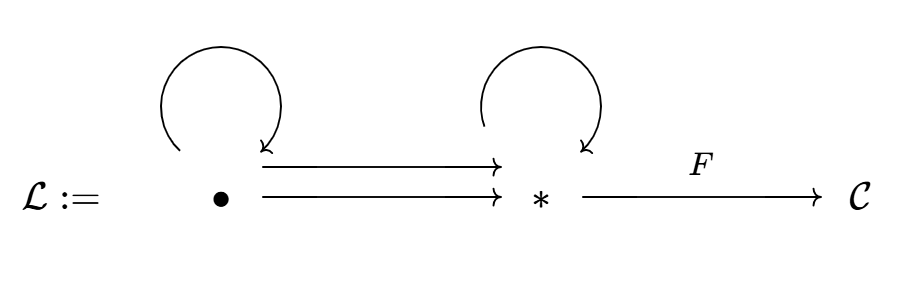
\includegraphics[width=0.5\linewidth]{img/diagrama6.png}
        \end{figure}
        Así, el límite sobre $\F$ de la forma $\L$ es 
        \begin{figure}[H]
            \centering
            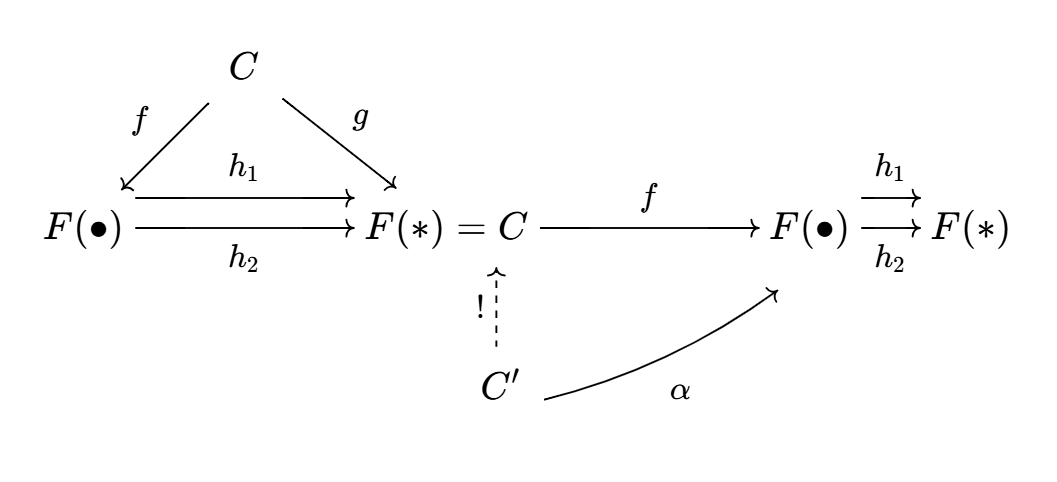
\includegraphics[width=0.6\linewidth]{img/diagrama7.png}
        \end{figure}
        Del diagrama anterior se tiene que, $g=h_1\circ f=h_2\circ f$. Por lo tanto, $C$ es el igualador de $F(\L)$.
        \item Sea $P$ la categoría que consiste de tres objetos $a$, $b$ y $c$, dos flechas $a\to b$, $b\to c$, y las respectivas identidades. Sea $F:P\to\C$ un funtor. En un diagrama se tiene que
        \begin{figure}[H]
            \centering
            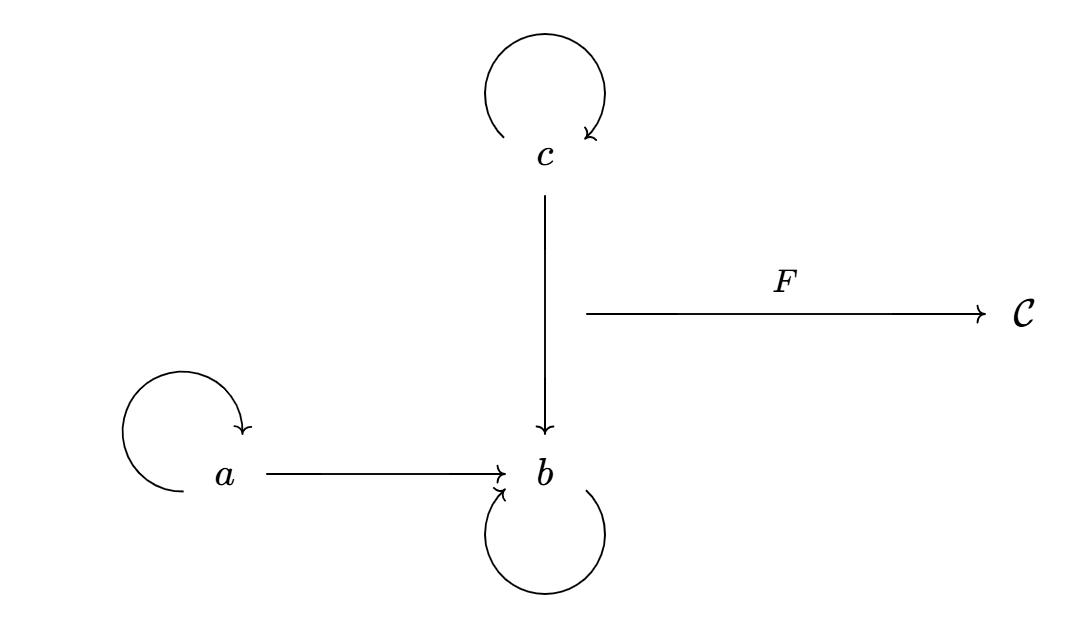
\includegraphics[width=0.6\linewidth]{img/diagrama8.png}
        \end{figure}
       Por lo cual, un límite sobre $F$ de la forma $P$ es el pullback
       \begin{figure}[H]
           \centering
           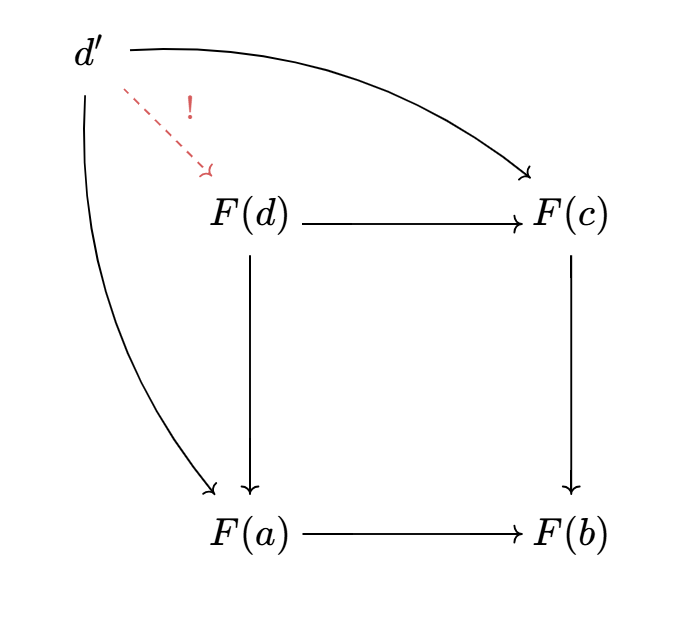
\includegraphics[width=0.38\linewidth]{img/diagrama9.png}
       \end{figure}
    \end{enumerate}
\end{ejp}
\subsection{Colímites}
\begin{definition}
    Sea $F:\A\to\C$ un funtor. Un \emph{cocono} sobre $F$ es una pareja  $(C,\langle s_A\rangle)_{A\in\A}$ que consiste de lo siguiente 
    \begin{enumerate}
        \item Un objeto $C\in \C$.
        \item Para cada $A\in\A$, un morfismo $(s_A:FA\to C)\in\C$ tal que, para cada flecha $\left(A\xrightarrow{\alpha}A'\right)\in\A$, el siguiente diagrama 
        \begin{figure}[h!]
            \centering
            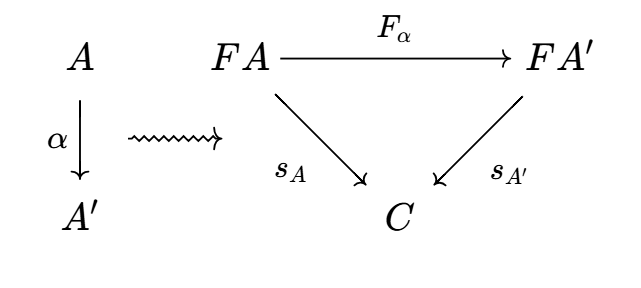
\includegraphics[width=0.4\linewidth]{img/diagrama3.png}
        \end{figure}
        conmuta en $\C$. Es decir, $s_A=s_{A'}\circ F_\alpha$.
    \end{enumerate}
\end{definition}
\begin{definition}
    Un \emph{colímite} sobre $F$ es un  cocono $(L,\langle s_A\rangle_{A\in\A})$ con la siguiente propiedad: para cualquier otro cocono $(M,\langle t_A\rangle_{A\in\A})$ el siguiente diagrama es conmutativo
    \begin{figure}[h!]
        \centering
        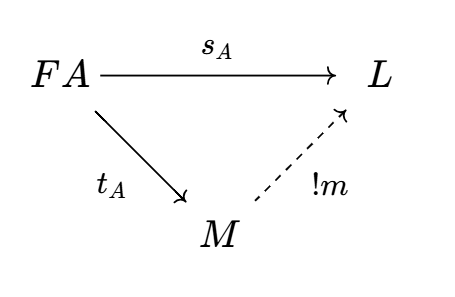
\includegraphics[width=0.3\linewidth]{img/diagrama4.png}
    \end{figure}
    Esto es, para todo $A\in \A$, $t_A=ms_A$.
\end{definition}
Por el principio de dualidad, los ejemplos de colímites se obtienen de manera dual a los ejemplos de límites dados en el Ejemplo \ref{ejp:lim}. 
\begin{lema}\label{lema:igualador}
    Sea $\left( A\xrightarrow{h}B \overset{f}{\underset{g}{\rightrightarrows}} C\right)\in\Con$. Este es un igualador si, y solo si, para cda $b\in B$ tal que $f(b)=g(b)$ implica que existe un único $a\in A$ tal que $h(a)=b$.
\end{lema}
\begin{proof}
    \todo{Pendiente}
\end{proof}
\begin{definition}
    Una categoría $\C$ es \emph{completa} si  cada funtor $F:\D\to\C$  tiene límite, donde $\D$ es una categoría pequeña. Dualmente, $\C$ es \emph{cocompleta} si todo funtor $F:\D\to\C$ tiene colímite. Si $\C$ es completa y cocompleta, diremos que es \emph{bicompleta.}
\end{definition}

\begin{lema}
    La categoría $\Con$ es bicompleta. En particular, los (co)límites de cada funtor se calculan puntualmente.
\end{lema}
\begin{proof}
    \todo{Pendiente}
\end{proof}

\begin{lema}
    Sea $(A,\leq)$ un conjunto parcialmente ordenado. Entonces, la categoría \begin{equation*}
    \Con^{(A,\leq)^{\op}}:[(A,\leq)^{\op},\Con]    
    \end{equation*} 
    es bicompleta y los (co)límites se calculan puntualmente.
\end{lema}
\begin{proof}
    \todo{Pendiente.}
\end{proof}
\begin{definition}
    Sea $\C$ una categoría pequeña.
    \begin{enumerate}
        \item[$\bullet$] Diremos que $\C$ es \emph{finita} si $\Ob(\C)$ y $\Mor(\C)$ son conjuntos finitos.
        \item[$\bullet$] Un límite sobre $F:\C\to \C'$ es \emph{finito} si $\C$ es finita. 
    \end{enumerate}
\end{definition}
\begin{definition}[Categoría filtrante]
    Una categoría $\C$ es \emph{filtrante} si
    \begin{enumerate}
        \item $\C$ es no vacía.
        \item Para cada $C_1, C_2\in \Ob(\C)$ existe $C\in \C$ junto con morfismos $C_1\xrightarrow{f_1} C$ y $C_2\xrightarrow{f_2} C$.
        \item Para cualesquiera $C_1,C_2\in \Ob(\C)$ y morfismos $C_1 \overset{f_1}{\underset{f_2}{\rightrightarrows}} C_2$ existe $C_3\in\Ob(\C)$ y un morfismo $C_1 \overset{f_1}{\underset{f_2}{\rightrightarrows}} C_2\xrightarrow{h} C_3$ tal que $hf_1=hf_2$.
    \end{enumerate}
\end{definition}
\begin{definition}
    Un \emph{colímite} sobre $F:\C\to\D$ es filtrante si $\C$ es filtrante.
\end{definition}
\begin{lema}
    Sea $F:\B\to\C$ un funtor con $\B$ finita y $\C$ filtrante. Entonces, existe un cono sobre $F$ en $\C$.
\end{lema}
La demostración se sigue del siguiente resultado. 
\begin{prop} Sea $\C$ una categoría pequeña.
    \begin{enumerate}
        \item Sea $\{C_i\mid i\in I\}$ un conjunto finito de objetos en $\C$. Entonces, podemos encontrar un objeto $C\in\C$ y morfismos $\{C_i\to C\mid i\in I\}$. 
        \item  Dado un conjunto finito $\{f_i:C\to C'\mid i\in I\}$, podemos encontrar un objeto $C''\in \C$ y un morfismo $C'\xrightarrow{f} C''$ tal que $ff_i=ff_j$, para todo $i,j\in I$. 
    \end{enumerate}
\end{prop}
\begin{proof}
    
\end{proof}
\section{Adjunciones}
\begin{definition}[Adjunción]
Sean $\C$ y $\D$ categorías. Una \emph{adjunción} entre $\C$ y $\D$ es una terna $(F,G,\varphi)$ donde $\D\overset{F}{\underset{G}{\rightleftarrows}}\C$ son funtores y $\varphi$ es una función que asigna a cada par de objetos $C\in\C$ y $D\in\D$ una biyección
\begin{equation*}
\varphi_{\D,\C}:\D(D,GC)\cong\C(FD,C).
\end{equation*}
En este caso, decimos  que $F$ es adjunto izquierdo y $G$ es adjunto derecho, lo cual es denotado por $F\dashv G$. 
\end{definition}
En lo anterior, $\varphi_{\D,\C}$ de hecho es un ismorfismo natural. El siguiente resultado nos dice que las adjunciones se comportan bien bajo composición.
\begin{lema}
    Sean $\D\overset{F}{\underset{G}{\rightleftarrows}}\C\overset{F'}{\underset{G'}{\rightleftarrows}}\B$ funtores. Si $F\dashv G$ y $F'\dashv G'$, entonces $F'\circ F\dashv G\circ G'$.
\end{lema}
\begin{proof}
    Como $F\dashv G$ se tiene que, para cada par de objetos $C\in \C$ y $D\in \D$, hay una biyección 
    \begin{eqnarray}\label{eq:1.7.1}
        \varphi_{\D,\C}:\D(D,GC)\cong\C(FD,C).
    \end{eqnarray}
    Del mismo modo, al ser $F'\dashv G'$, para cada par de objetos $C'\in C$ y $B\in \B$, existe una biyección
    \begin{equation}\label{eq:1.7.2}
        \varphi_{\C,\B}:\C(C, G'B)\cong\B(F'C', B).
    \end{equation}
    Si $D\in \D$ y $B\in \B$, al primero evaluar en (\ref{eq:1.7.1}) en los objetos $C$ y $G'B\in \C$, y después evaluar (\ref{eq:1.7.2}) en $FC\in\D$ y $B\in \B$, obtenemos
    \begin{eqnarray*}
        \D(D,G(G'B))\cong \C(FD,G'B)\cong\B(F'(FC),B).
    \end{eqnarray*}
    Por lo tanto, $F'\circ F\dashv G\circ G'$ tal como se quería.
\end{proof}
A continuación se enuncian un par de resultados en los que se muestra la relación entre objetos iniciales/finales y adjuntos. Esto es, si una categoría tiene objeto inicial, este da lugar a un adjunto izquierdo. Dualmente, si la categoría tiene objeto  final, este determina un adjunto derecho.
\begin{prop}
    Si $\A$ y $\B$ son categorías con objeto inicial entonces el funtor 
    \begin{eqnarray*}
    \sigma_\A:\A&\to&\A\times \B\\
    A&\mapsto& (A,0)\\
    f&\mapsto& (f,1_0)
  \end{eqnarray*}
  es adjunto izquierdo de la proyección $\pi_\A:\A\times\B\to\A$.
\end{prop}
\begin{prop}
    Sean $\A$, $\B$ y $\C$ categorías con coproductos finitos y funtores 
    \begin{figure}[H]
        \centering
        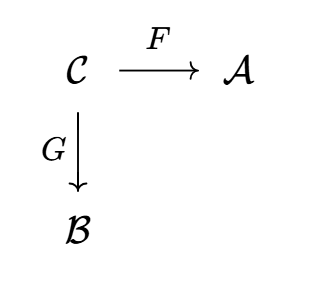
\includegraphics[width=0.18\linewidth]{img/diagram1.4.1.png}
    \end{figure}
    Entonces, el funtor $\langle F,G\rangle:\C\to\A\times\B$ si, y solo si, ambos funtores $F$ y $G$ tienen adjunto izquierdo.
\end{prop}
Ahora, considereos $\C$ y $\D$ dos categorías y $\D\overset{F}{\underset{G}{\rightleftarrows}}\C$ funtores. Si $\left(D\xrightarrow{h}D'\right)\in\D$ y $\left(C\xrightarrow{k}C'\right)\in \D$, de la definición de adjunción, se tienen los siguientes diagramas conmutativos.
    \begin{figure}[H]
        \centering
        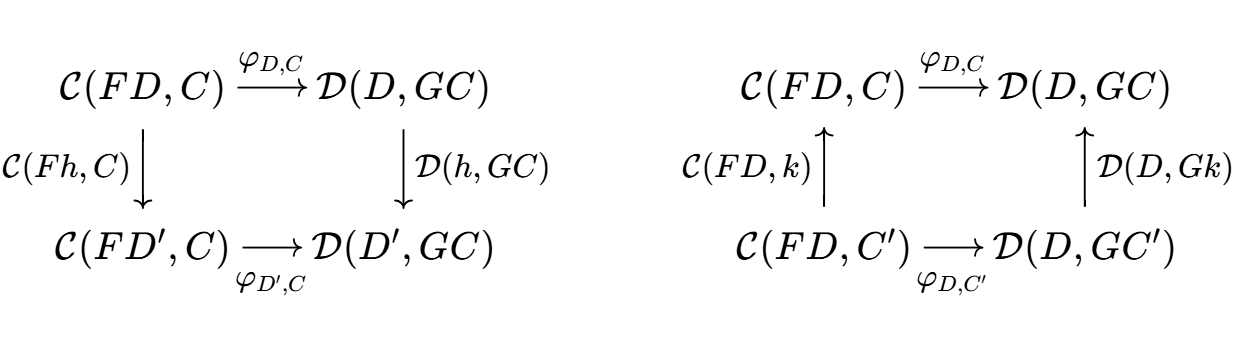
\includegraphics[width=0.8\linewidth]{img/diagram1.4.2.png}
    \end{figure}
    En otras palabras, para todo $FD\xrightarrow{f}C$ se tiene que $\varphi(f\circ Fh)=\varphi(f)h$ y $\varphi(k\circ f)=Gk\circ\varphi f$. Esto es equivalentea que $\varphi^{-1}$ sea también un isomorfismo natural. Es decir, con las mismas flechas y $D'\xrightarrow{g} GC$, se tiene que $\varphi^{-1}(gh)=\varphi^{-1}gFh$ y $\varphi^{-1}(Gkg)=k\varphi^{-1}(g)$. \\
    Tomando el caso particular $C=FD$, se tiene el diagrama conmutativo.
        \begin{figure}[H]
        \centering
        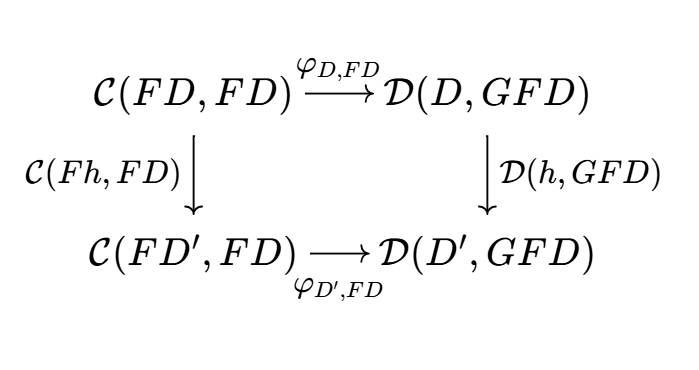
\includegraphics[width=0.45\linewidth]{img/diagram1.4.3.png}
    \end{figure}
    \text{}\\
    Defina $\eta_D=\varphi(1_{FD}):D\to GFD$, para toda $D\in \D$.\\
    \emph{Afirmación. } $\langle \eta_D\mid D\in\D\rangle$ define una transformación natural $\eta:1_D\to GF$. \\
    Basta verificar que el siguiente diagrama conmuta
        \begin{figure}[H]
        \centering
        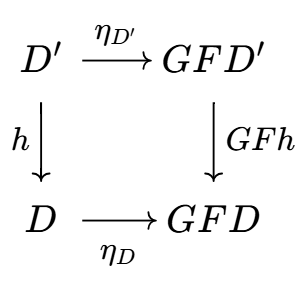
\includegraphics[width=0.2\linewidth]{img/diagram1.4.4.png}
    \end{figure}
    Lo cual es inmediata ya que 
    \begin{equation*}
        GF\varphi(1_D)=\varphi(Fh)=\varphi(1_{D'})h.
    \end{equation*}
    A esta transformación natural $\eta_D:1_D\to GF$ se le llama \emph{unidad de la adjunción} $(F,G,\varphi):\D\to\C$.\\
    Por otro lado, consideremos el caso particular $D=GC$. Entonces se tiene el siguiente diagrama conmutativo. 
           \begin{figure}[H]
        \centering
        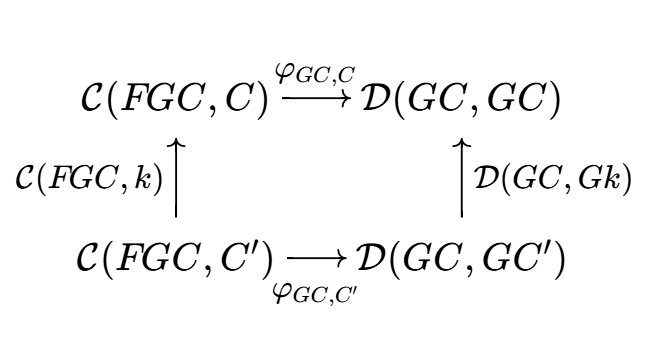
\includegraphics[width=0.45\linewidth]{img/diagram1.4.5.png}
    \end{figure}
    Se define $\varepsilon_C$ como $\phi^{-1}(1_{GA}):FGC\to C$, para toda $C\in \C$. De manera similar a como se hizo con $\eta_D$, se puede verificar que $\epsilon_C$ es una transformación natural, a la cual le llamamos \emph{counidad de la adjunción} $(F,G,\phi): \D\to \C$.
    \begin{definition}[Equivalencia de categorías]
        Dos categorías $\C$ y $\D$ son \emph{equivalentes} si existe una adjunción $(F,G, \eta,\varepsilon):\D\to\C$ tal que la unidad y la counidad son isomorfismos naturales. En este caso, decimos que los funtores $F$ y $G$ son una equivalencia de categorías. 
    \end{definition}
    Para finalizar, veremos una ``aplicación'' de los conceptos vistos en esta sección para el caso particular cuando las categorías son retículas. Dado un conjunto parcialmente ordenado $(A,\leq)$, se dice que es una \emph{retícula} si cada subconjunto finito no vacío $X\subseteq A$ tiene supremo e ínfimo.
    \begin{lema}
    Sean $(A,\leq)$ y $(B,\leq)$ retículas. El funtor $F:\A\to\B$ tiene adjunto derecho si, y solo si, $F$ preserva supremos arbitrarios.     
    \end{lema}
    \begin{proof}\text{}\\
    $\boxed{\Longrightarrow}$
        Supongamos que existe un funtor $G:\B\to \A$ tal que $F\dashv G$. Lo anterior ocurre si, y solo  si, 
        \begin{equation}\label{eq:1.4.1}
            A\leq GB\iff FA\leq B, \quad\forall A\in \Ob(\A), B\in\Ob(\B).
        \end{equation}
        Sea $\bigvee_{i\in I} A_i$ un supremo en $\A$. Esto es, $A\leq \bigvee_{i\in I} A_i$. Dado que $F$ es un funtor, $FA_i\leq F\left(\bigvee_{i\in I}A_i\right)$. Luego, 
        \begin{eqnarray*}
            FA_i\leq \bigvee_{i\in I}FA_i\leq F\left(\bigvee_{i\in I}A_i\right).
        \end{eqnarray*}
        Por (\ref{eq:1.4.1}), se tiene que 
        \begin{eqnarray*}
           A_i\leq G\left(\bigvee_{i\in I}F A_i\right).
        \end{eqnarray*}
        Así, $\bigvee_{i\in I}A_i\leq G\left(\bigvee_{i\in I}FA_i\right)$. Nuevamente, por (\ref{eq:1.4.1}), 
        \begin{eqnarray*}
        F\left(\bigvee_{i\in I}A_i\right)\leq \bigvee_{i\in I}FA_i.
        \end{eqnarray*}
        Ya que se tiene la doble desigualdad, se concluye que $F\left(\bigvee_{i\in I}A_i\right)=\bigvee_{i\in I} FA_i$.\\
        $\boxed{\Longleftarrow}$. Ahora, supongamos que $F$ preserva supremos arbitrarios. Sea $B\in\Ob(\B)$ y tomemos $GB=\bigvee_{FA\leq B}A$. Si $B'\in\Ob(\B)$ es tal que $B'\leq B$, entonces $F(A)\leq B'$ implica que $F(A)\leq B$. Así, 
        \begin{eqnarray*}
            GB'=\bigvee_{FA\leq B'} A\leq\bigvee_{FA\leq B} A=GB
        \end{eqnarray*}
        y $G:\B\to\A$ es funtorial. Ahora, resta probar que $A\leq GB$ si, y solo si $FA\leq B$. Para esto, consideremos $A\in\Ob(\A)$ y $B\in\Ob(\B)$. Si $A\leq GB$, entonces $A\leq\bigvee_{FA\leq B}A$. En virtud de que $F$ preserva supremos arbitrarios, 
        \begin{eqnarray*}
            FA\leq \bigvee_{FA\leq B}FA\leq B.
        \end{eqnarray*}
        Por otro lado, si $FA\leq B$, al ser $G$ un funtor, se tiene que $GFA\leq GB$. Luego, 
        \begin{eqnarray*}
            A=\bigvee_{FA'\leq FA}A'\leq GB
        \end{eqnarray*}
        tal como se quería.
    \end{proof}
\section{Extensiones de Kan}
Recordemos que $\Fun(\A,\B)$ denota la categoría de funtores de la categoría $\A$ en la categoría $\B$, y cuyos morfismos son las transformaciones naturales entre ellos. Lo que se desea probar en esta sección es que la precomposición 
\begin{eqnarray*}
-\circ F:\Fun(\B,\C)&\to&\Fun(\A,\C)\\
G&\mapsto& G\circ F
\end{eqnarray*}
tiene adjunto izquierdo si $\C$ es cocompleta. Como caso particular, esto ocurre si $\C=\Con$.
\begin{definition}[Extensión de Kan]
    Sean $F:\A\to \B$  y $G:\B\to \C$ funtores. La \emph{extensión de Kan izquierdad} de $G$ a lo largo de $F$, si existe, es una pareja $(K:\B\to\C,\text{ }\alpha:G\Rightarrow K\circ F)$, donde $K$ es un funtor y $\alpha$ una transformación natural, que es universal: para cualquier otra pareja $(H:\B\to\C,\text{ }\beta: G\Rightarrow H\circ F )$ existe una única transformación natural $\gamma: K\Rightarrow H$ tal que $(\gamma\circ F)\alpha=\beta$. Es decir, el diagrama 
    \begin{figure}[H]
        \centering
        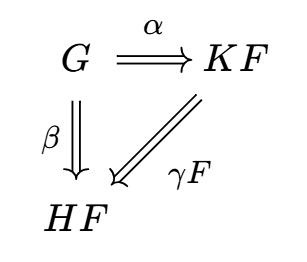
\includegraphics[width=0.2\linewidth]{img/diagram1.4.6.png}
    \end{figure}
    conmuta. El funtor $K$ es denotado por $\Lan_F G$.
\end{definition}
\begin{theo}
    Sean $F:\A\to\B$ y $G:\B\to\C$ funtores. Si $\A$ es pequeña, y $\C$ es cocompleta, entonces la extensión de Kan izquierda de $G$ a lo largo de $F$ existe.
\end{theo}
\begin{proof}
    \todo{Pendiente.}
\end{proof}
Sean $\A$ y $\B$ categorías pequeñas y $\C$ una categoría cocompleta. Consideremos el funtor $-\circ F:\Fun(\B,\C)\to\Fun(\A,\C)$ dado por 
    \begin{figure}[H]
        \centering
        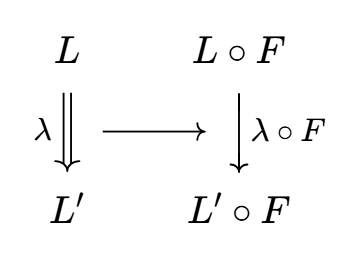
\includegraphics[width=0.25\linewidth]{img/diagram1.4.7.png}
    \end{figure}
Ahora, definimos el funtor $\Lan_{F_{-}}:\Fun(\A,\C)\to\Fun(\B,\C)$
como
    \begin{figure}[H]
        \centering
        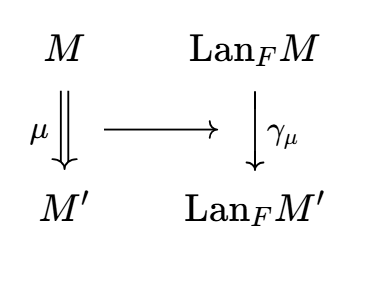
\includegraphics[width=0.25\linewidth]{img/diagram1-4-8.png}
    \end{figure}

donde $\Lan_F M$ es el funtor de la pareja $(\Lan_FM:\B\to\C,\text{ }\alpha_M: M\Rightarrow \Lan_FM\circ F)$. Para culaquier otra pareja $(\Lan_F M':\B\to\C,\text{ }\alpha_{M'}\circ\mu:M\Rightarrow \Lan_F M'\circ F)$, se tiene que $\gamma_\mu:\Lan_F M\Rightarrow \Lan_F M'$ es la única transformación natural tal que $(\gamma_\mu\circ F)\alpha_M=\alpha_{M'}$. Así, se tiene el siguiente resultado. 
\begin{prop}
    Sea $F:\A\to\B$ un funtor y $\C$ una categoría. Si $\A$ es pequeña y $\C$ es cocompleta, entonces $\Lan_{F_{-}}$ es adjunto izquierdo de $-\circ F$.
\end{prop}
\begin{proof}
    \todo{Pendiente.}
\end{proof}
\section{Categorías extensivas}
A lo largo de esta sección, nos referiremos a coproductos finitos como sumas finitas. Para tener una descripción detallada de las demostraciones se sugiere al lector interesado en consultar \cite{Merino2002}.
Dada una categoría $\E$ que admite sumas finitas, y cualesquiera dos objetos $A$ y $B$ de $\E$, se construye la categoría $\E/A\times\E/B $ cuyos objetos son pares $(f,g)$ donde $f:A'\to A$ y $g:B'\to B$, para todo $A', B'\in \Ob(\E)$. Mientras que los morfismos son parejas $(\alpha,\beta)$ donde $\alpha:A'\to A''$ es tal que $f=f'\circ\alpha$, con $f':A''\to A'$ para todo $A', A''$, y lo mismo con $\beta$. A partir de la categoría $\E/A\times\E/B$ se puede construir un funtor que vaya a la categoría $\E/A+B$, esto motiva la siguiente definición.
\begin{definition}
    Sea $\E$ una categoría con sumas finitas y, $A$ y $B$ un par de objetos en $\E$. Se define el funtor 
    \begin{eqnarray*}
        +:\E/A\times\E/B\to\E/A+B
    \end{eqnarray*}
    como aquel que para cada $(f,g)\in\Ob(\E/A\times\E/B)$ le asigna una flecha inducida por la suma. En un diagrama, esto es
    \begin{figure}[H]
        \centering
        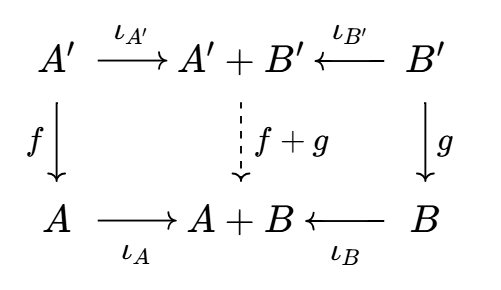
\includegraphics[width=0.35\linewidth]{img/diagrama1.5.1.png}
    \end{figure}
    Mientras que a cada morfismo $(\alpha,\beta)$ en $\E/A\times\E/B$ también le asigna la flecha inducida por la suma tal como lo muestra el siguiente diagrama.
        \begin{figure}[H]
        \centering
        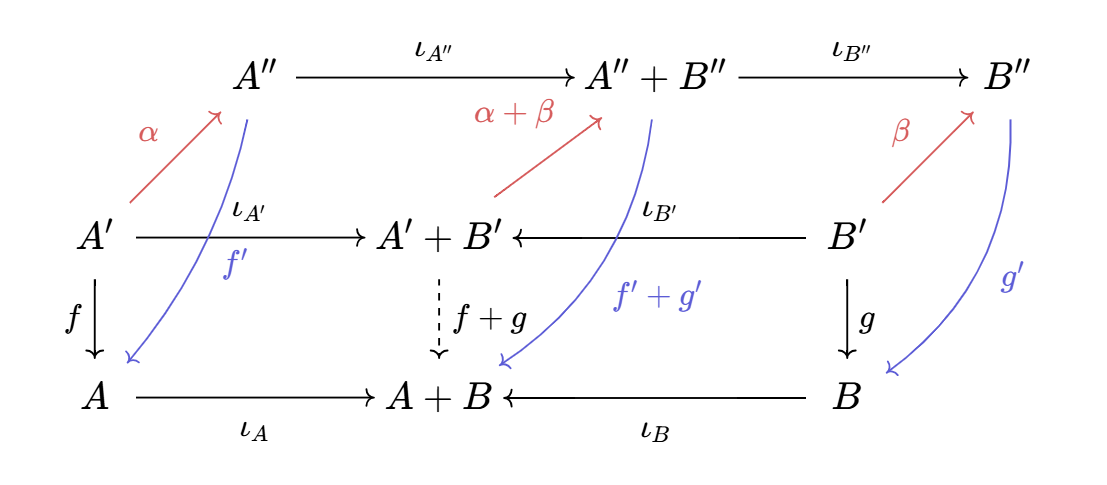
\includegraphics[width=0.75\linewidth]{img/diagram1.5.2.png}
    \end{figure}
\end{definition}
\begin{definition}[Categoría extensiva]
    Sea $\E$ una categoría con sumas finitas. Decimos que $\E$ satisface la \emph{ley extensiva} si, para cada par de objetos $A$ y $B$ de $\E/A\times \E/B$, el funtor $+:\E/A\times\E/B\to\E/A+B$ es una equivalencia de categorías. En este caso, diremos que $\E$ es una categoría extensiva. 
\end{definition}
A grandes rasgos, uno puede pensar en una categoría extensiva como aquella en la que los coproductos (sumas finitas en nuestro caso) se ``comportan bien'' con cierta clase de pullbacks. 
\begin{ejp}
\text{}
    \begin{enumerate}
        \item $\Con$ es extensiva.
        \item $\Top$ es extensiva.
        \item Si $\C$ es una categoría pequeña, entonces la categoría $\mathrm{Fun}[\C^\op,\Con]$ es extensiva.
        \item La categoría de espacios vectoriales sobre un campo $k$, $\Vect_k$, no es extensiva (el coproducto es la suma directa).
    \end{enumerate}
\end{ejp}
\begin{definition}[Sumas universales]
    Dada una categoría $\E$ que admite sumas finitas, diremos que las sumas son \emph{universales} si, para cualquier morfismo $f:S\to A+B$, los productos fibrados a lo largo de las inyecciones existen y el renglón superior del siguiente diagrama
        \begin{figure}[H]
        \centering
        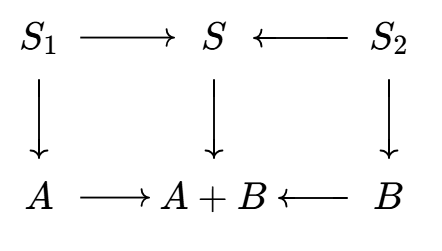
\includegraphics[width=0.3\linewidth]{img/diagrama1.5.3.png}
    \end{figure}
    es una suma. 
\end{definition}
\begin{definition}
    Si una categoría $\E$ tiene objeto inicial $A$, se dice que $A$ es \emph{estricto} si para cada flecha $A\to 0$ se tiene que $A=0$. 
\end{definition}
\begin{lema}
    Si $\E$ es una suma con sumas universales, ebtobces el objeto inicial es estricto.
\end{lema}
\begin{theo}
    Sea $\E$ una categoría con sumas universales. Entonces, $\E$ es extensiva si, y solo si, satisface lo siguiente.
    \begin{enumerate}
        \item[i)] Para cualquier diagrama conmutativo de la forma
        \begin{figure}[H]
        \centering
        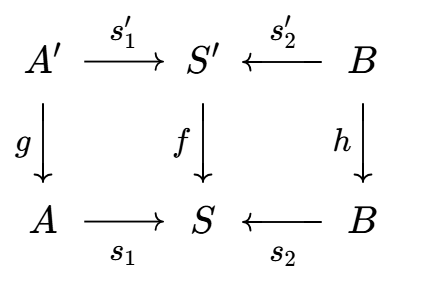
\includegraphics[width=0.3\linewidth]{img/diagrama1.5.4.png}
        \end{figure}
        tal que el renglón inferior es una suma, cumple que el renglón superior también es una suma, entonces ambos cuadrados son productos fibrados.
        \item[ii)] Toda suma en $\E$ es universal.
    \end{enumerate}
\end{theo}